\subsection{Выборочные коэффициенты корреляции}
\begin{table}[H]
	\centering
	\begin{tabular}{| c | c | c | c |}
		
		\hline
		$\rho=0$  & $r$      & $r_S$  & $r_Q$ \\
		\hline
        $E(z)$   & -0.0102 & -0.012 & 0.0   \\
        $E(z^{2})$  & 0.023 & 0.024 & 0.04  \\
        $D(z)$   & 0.054 & 0.054 & 0.0544 \\
		\hline
		$\rho=0.5$ & $r$      & $r_S$  & $r_Q$ \\
		\hline
		$E(z)$      & 0.51 & 0.47 & 0.4   \\
        $E(z^{2})$   & 0.26 & 0.23 & 0.16  \\
        $D(z)$     & 0.033 & 0.036 & 0.047 \\
		\hline
		$\rho=0.9$  & $r$      & $r_S$  & $r_Q$ \\
		\hline
		$E(z)$      & 0.9 & 0.87 & 0.7   \\
        $E(z^{2})$   & 0.81 & 0.76 & 0.5  \\
        $D(z)$      & 0.0025 & 0.0051 & 0.0294 \\
		\hline
		
	\end{tabular}{}
	\caption{Двумерное нормальное распределение, n = 20}
	\label{tab:n20}
\end{table}
\begin{table}[H]
	\centering
	\begin{tabular}{| c | c | c | c |}
		
		\hline
		$\rho = 0$ & $r$      & $r_S$  & $r_Q$ \\
		\hline
		$E(z)$     & -0.004 & -0.007 & 0.0   \\
        $E(z^{2})$  & 0.007 & 0.008 & 0.004 \\
        $D(z)$    & 0.017 & 0.016 & 0.016 \\
		\hline
		$\rho = 0.5$ & $r$      & $r_S$  & $r_Q$ \\
		\hline
		$E(z)$      & 0.498 & 0.477 & 0.333 \\
        $E(z^{2})$    & 0.248 & 0.227 & 0.111 \\
        $D(z)$      & 0.01 & 0.01 & 0.014 \\
		\hline
		$\rho = 0.9$ & $r$      & $r_S$  & $r_Q$ \\
		\hline
		$E(z)$      & 0.903 & 0.888 & 0.733 \\
        $E(z^{2})$    & 0.815 & 0.789 & 0.537 \\
        $D(z)$      & 0.0007 & 0.0011 & 0.008 \\
		\hline
		
	\end{tabular}{}
	\caption{Двумерное нормальное распределение, n = 60}
	\label{tab:n60}
\end{table}

\begin{table}[H]
	\centering
	\begin{tabular}{| c | c | c | c |}
		
		\hline
		$\rho = 0$ & $r$      & $r_S$  & $r_Q$ \\
		\hline
		$E(z)$    & 0.003 & -0.001 & 0.0   \\
        $E(z^{2})$  & 0.004 & 0.004 & 0.006 \\
        $D(z)$    & 0.0095 & 0.0097 & 0.0099 \\
		\hline
		$\rho = 0.5$ & $r$      & $r_S$  & $r_Q$ \\
		\hline
		$E(z)$      & 0.494 & 0.475 & 0.32  \\
        $E(z^{2})$    & 0.244 & 0.225 & 0.102 \\
        $D(z)$      & 0.005 & 0.006 & 0.008 \\
		\hline
		$\rho = 0.9$ & $r$      & $r_S$  & $r_Q$ \\
		\hline
		$E(z)$      & 0.9 & 0.89 & 0.72  \\
        $E(z^{2})$    & 0.811 & 0.792 & 0.518 \\
        $D(z)$      & 0.0004 & 0.0007 & 0.0052 \\
		\hline
		
	\end{tabular}{}
	\caption{Двумерное нормальное распределение, n = 100}
	\label{tab:n100}
\end{table}


\begin{table}[H]
	\centering
	\begin{tabular}{| c | c | c | c |}
		
		\hline
		$N = 20$ & $r$      & $r_{S}$ & $r_{Q}$ \\
		\hline
		$E(z)$      & 0.796 & 0.763 & 0.6   \\
        $E(z^{2})$     & 0.633 & 0.583 & 0.36 \\
        $D(z)$      & 0.008 & 0.011 & 0.035 \\
		\hline
		$N = 60$ & $r$      & $r_{S}$ & $r_{Q}$ \\
		\hline
		$E(z)$      & 0.796 & 0.776 & 0.6   \\
        $E(z^{2})$    & 0.634 & 0.602 & 0.36  \\
        $D(z)$      & 0.0026 & 0.0036 & 0.011 \\
		\hline
		$N = 100$ & $r$      & $r_{S}$ & $r_{Q}$ \\
		\hline
		$E(z)$       & 0.793 & 0.774 & 0.56   \\
        $E(z^{2})$     & 0.629 & 0.599 & 0.313  \\
        $D(z)$      & 0.001 & 0.002 & 0.006 \\
		\hline
		
	\end{tabular}{}
	\caption{Смесь нормальных распределений}
	\label{tab:mix_normal}
\end{table}


\subsection{Эллипсы рассеивания}
\noindent Для уравнения эллипса выбиралась константа равная $const = 2 \cdot (2 \cdot \sigma)$

\begin{figure}[H]
	\centering
	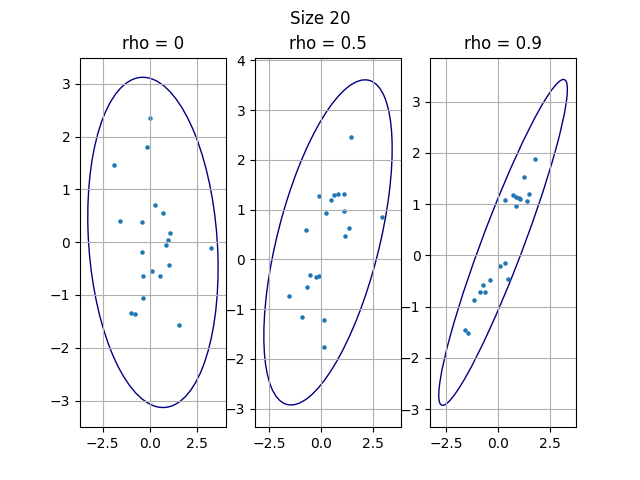
\includegraphics[width = 16cm, height = 10cm]{res/size20_t1.png}
	\caption{Двумерное нормальное распределение, $n$ = 20}
	\label{fig:n20}
\end{figure}

\begin{figure}[H]
	\centering
	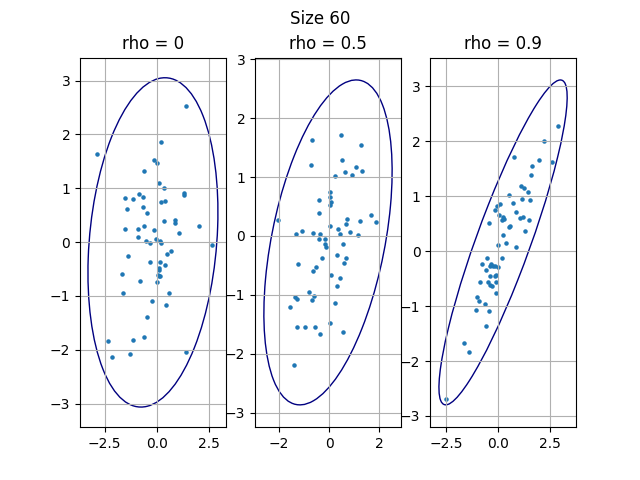
\includegraphics[width = 16cm, height = 10cm]{res/size60_t1.png}
	\caption{Двумерное нормальное распределение, $n$ = 60}
	\label{fig:n60}
\end{figure}

\begin{figure}[H]
	\centering
	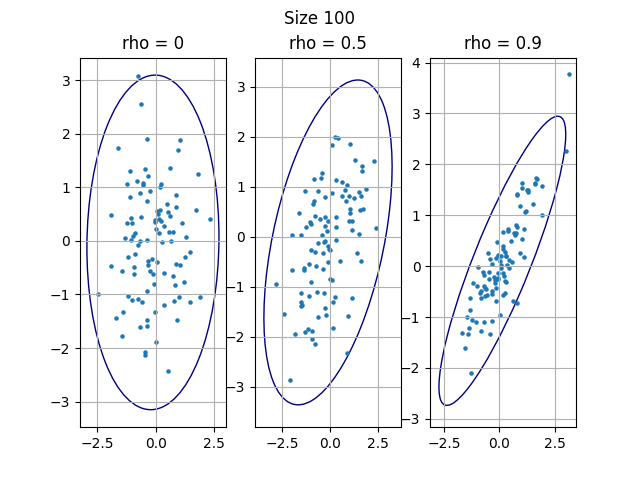
\includegraphics[width = 16cm, height = 10cm]{res/size100_t1.png}
	\caption{Двумерное нормальное распределение, $n$ = 100}
	\label{fig:n100}
\end{figure}


%% Вторая работа
\subsection{Оценки коэффициентов линейной регрессии}
\subsubsection{Выборка без возмущений}
	\begin{itemize}
		\item{Критерий наименьших квадратов:}
		$\hat{a}\approx 1.89$, $\hat{b}\approx 1.73$
		\item{Критерий наименьших модулей:}
		$\hat{a}\approx 1.85$, $\hat{b}\approx 1.51$
	\end{itemize}
	\begin{figure}[H]
		\centering
		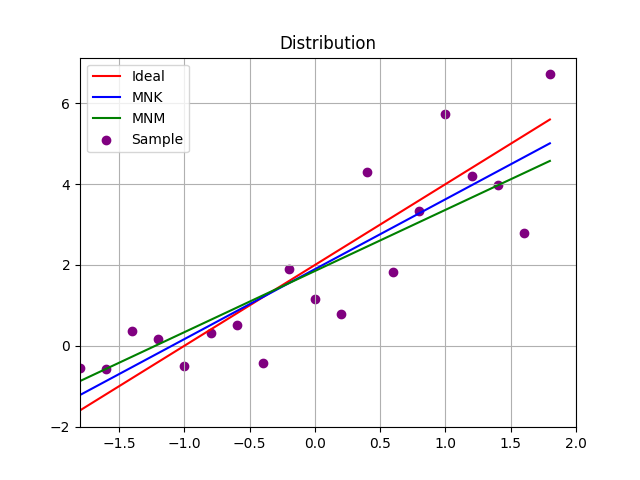
\includegraphics[width = 12cm, height = 10cm]{res/distr_t2.png}
		\caption{Выборка без возмущений}
		\label{w/o_pert}
	\end{figure}

\subsubsection{Выборка с возмущениями}
	\begin{itemize}
		\item{Критерий наименьших квадратов:}
		$\hat{a}\approx 1.89$, $\hat{b}\approx 0.2$
		\item{Критерий наименьших модулей:}
		$\hat{a}\approx 1.17$, $\hat{b}\approx 1.07$
	\end{itemize}
	\begin{figure}[H]
		\centering
		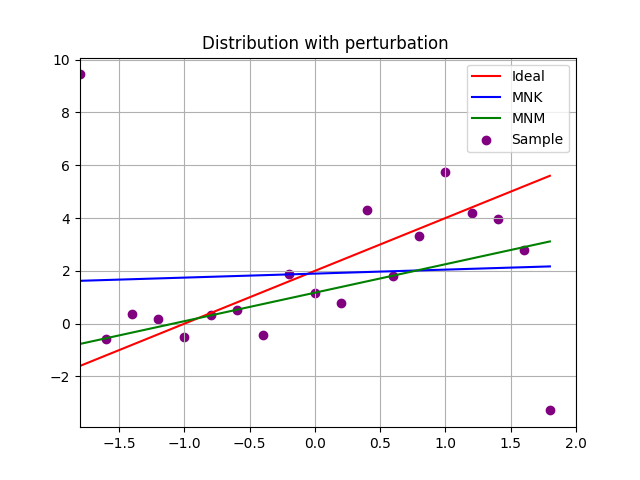
\includegraphics[width = 12cm, height = 10cm]{res/distr_pert_t2.png}
		\caption{Выборка с возмущениями}
		\label{w_pert}
	\end{figure}


%% Третья работа
\subsection{Проверка гипотезы о законе распределения генеральной совокупности. Метод хи-квадрат}
    
\noindent 
\centering
\begin{cases}
& $\mu = -0.04$ \\
& $\sigma = 1.17$\\
& $\chi^{2}_{0.95} \approx 14.07$\\
& $k = 5$
\end{cases}\\
\begin{table}[H]
    \centering
\begin{tabular}{| c | c | c | c | c | c | c |}
\hline
    $i$ & $limits$         &   $n_i$ &    $p_i$ &   $np_i$ &   $n_i - np_i$ &   $\frac{(n_i-np_i)^2}{np_i}$ \\
\hline
   1 & [-inf, -1.1]       &    22 & 0.1357 &  13.5666 &       8.4334 &                      5.2424 \\
   2 & [-1.1, -0.7333]    &     6 & 0.096  &   9.6012 &      -3.6012 &                      1.3507 \\
   3 & [-0.7333, -0.3667] &    10 & 0.1253 &  12.5256 &      -2.5256 &                      0.5093 \\
   4 & [-0.3667, 0.0]     &    10 & 0.1431 &  14.3066 &      -4.3066 &                      1.2964 \\
   5 & [0.0, 0.3667]      &    13 & 0.1431 &  14.3066 &      -1.3066 &                      0.1193 \\
   6 & [0.3667, 0.7333]   &    13 & 0.1253 &  12.5256 &       0.4744 &                      0.018  \\
   7 & [0.7333, 1.1]      &    11 & 0.096  &   9.6012 &       1.3988 &                      0.2038 \\
   8 & [1.1, 'inf']       &    15 & 0.1357 &  13.5666 &       1.4334 &                      0.1514 \\
   $\sum$ & -                  &   100 & 1      & 100      &      -0      &                      8.8913 \\
\hline
\end{tabular}
\caption{ Вычисление $\chi^{2}_{B}$ при нормальном законе распределения $N(x,\hat{\mu}, \hat{\sigma})$}
\label{tab:normal_chi_2}
\end{table}

\noindent 
\centering
\begin{cases}
& $\mu = 0.3$ \\
& $\sigma = 0.65$\\
& $\chi^{2}_{0.95} \approx 9.48$\\
& $k = 5$
\end{cases}\\
\begin{table}[H]
    \centering
\begin{tabular}{| c | c | c | c | c | c | c |}
\hline
		$i$ & $limits$         &   $n_i$ &    $p_i$ &   $np_i$ &   $n_i - np_i$ &   $\frac{(n_i-np_i)^2}{np_i}$ \\
\hline
   1 & [-inf, -1.1]      &     0 & 0.1357 &  2.7133 &      -2.7133 &                      2.7133 \\
   2 & [-1.1, -0.3667]   &     3 & 0.2213 &  4.4254 &      -1.4254 &                      0.4591 \\
   3 & [-0.3667, 0.3667] &     9 & 0.2861 &  5.7226 &       3.2774 &                      1.8769 \\
   4 & [0.3667, 1.1]     &     4 & 0.2213 &  4.4254 &      -0.4254 &                      0.0409 \\
   5 & [1.1, 'inf']      &     4 & 0.1357 &  2.7133 &       1.2867 &                      0.6102 \\
   $\sum$ & -                 &    20 & 1      & 20      &      -0      &                      5.7004 \\
\hline
\end{tabular}
\caption{ Вычисление $\chi^{2}_{B}$ при распределении Лапласа $L(x,\hat{\mu}, \hat{\sigma})$}
\label{tab:laplace_chi_2}
\end{table}

\noindent 
\centering
\begin{cases}
& $\mu = 0.72$ \\
& $\sigma = 0.93$\\
& $\chi^{2}_{0.95} \approx 9.48$\\
& $k = 5$
\end{cases}\\
\begin{table}[H]
    \centering
\begin{tabular}{| c | c | c | c | c | c | c |}
\hline
		$i$ & $limits$         &   $n_i$ &    $p_i$ &   $np_i$ &   $n_i - np_i$ &   $\frac{(n_i-np_i)^2}{np_i}$ \\
\hline
   1 & [-inf, -1.1]      &     2 & 0.1357 &  2.7133 &      -0.7133 &                      0.1875 \\
   2 & [-1.1, -0.3667]   &     1 & 0.2213 &  4.4254 &      -3.4254 &                      2.6513 \\
   3 & [-0.3667, 0.3667] &     3 & 0.2861 &  5.7226 &      -2.7226 &                      1.2953 \\
   4 & [0.3667, 1.1]     &     5 & 0.2213 &  4.4254 &       0.5746 &                      0.0746 \\
   5 & [1.1, 'inf']      &     9 & 0.1357 &  2.7133 &       6.2867 &                     14.566  \\
   $\sum$ & -                 &    20 & 1      & 20      &      -0      &                     18.7749 \\
\hline
\end{tabular}
    \caption{ Вычисление $\chi^{2}_{B}$ при равномерном распределении $U(x,\hat{\mu}, \hat{\sigma})$}
    	\label{tab:unifrom_chi_2}
\end{table}


%% Четвертая работа
\subsection{Доверительные интервалы для параметров нормального распределения}
	\begin{table}[H]
	    \centering
	    \begin{tabular}{| c | c | c |}
	    \hline
	       n = 20   &  $m$  & $\sigma$\\ \hline
	          &  -0.41 < $m$ < 0.5 & 0.74 < $\sigma$ < 1.43 \\ \hline
	         &   &   \\ \hline
	       n = 100   &  $m$  & $\sigma$\\ \hline
	        & -0.09 < $m$ < 0.25 & 0.75 < $\sigma$ < 1.0 \\
	   \hline
	    \end{tabular}
	    \caption{Доверительные интервалы для параметров нормального распределения}
	    \label{tab:interv_simple}
	\end{table}
	
\subsection{Доверительные интервалы для параметров произвольного распределения. Асимптотический подход}
	\begin{table}[H]
	    \centering
	    \begin{tabular}{| c | c | c |}
	    \hline
	       n = 20   &  $m$  & $\sigma$\\ \hline
	          &  -0.39 < $m$ < 0.48 & 0.76 < $\sigma$ < 1.46 \\ \hline
	         &   &   \\ \hline
	       n = 100   &  $m$  & $\sigma$\\ \hline
	        & -0.11 < $m$ < 0.27 & 0.76 < $\sigma$ < 0.99 \\
	   \hline
	    \end{tabular}
	    \caption{Доверительные интервалы для параметров произвольного распределения. Асимптотический подход}
	    \label{tab:interv_asimpt}
	\end{table}
	